% Options for packages loaded elsewhere
\PassOptionsToPackage{unicode}{hyperref}
\PassOptionsToPackage{hyphens}{url}
\PassOptionsToPackage{dvipsnames,svgnames,x11names}{xcolor}
%
\documentclass[
  11pt,
]{book}
\title{Dispense sull'analisi delle componenti principali}
\usepackage{etoolbox}
\makeatletter
\providecommand{\subtitle}[1]{% add subtitle to \maketitle
  \apptocmd{\@title}{\par {\large #1 \par}}{}{}
}
\makeatother
\subtitle{Principal Component Analysis, PCA}
\author{Giorgio Marrubini e Camillo Melzi}
\date{}

\usepackage{amsmath,amssymb}
\usepackage{lmodern}
\usepackage{iftex}
\ifPDFTeX
  \usepackage[T1]{fontenc}
  \usepackage[utf8]{inputenc}
  \usepackage{textcomp} % provide euro and other symbols
\else % if luatex or xetex
  \usepackage{unicode-math}
  \defaultfontfeatures{Scale=MatchLowercase}
  \defaultfontfeatures[\rmfamily]{Ligatures=TeX,Scale=1}
\fi
% Use upquote if available, for straight quotes in verbatim environments
\IfFileExists{upquote.sty}{\usepackage{upquote}}{}
\IfFileExists{microtype.sty}{% use microtype if available
  \usepackage[]{microtype}
  \UseMicrotypeSet[protrusion]{basicmath} % disable protrusion for tt fonts
}{}
\makeatletter
\@ifundefined{KOMAClassName}{% if non-KOMA class
  \IfFileExists{parskip.sty}{%
    \usepackage{parskip}
  }{% else
    \setlength{\parindent}{0pt}
    \setlength{\parskip}{6pt plus 2pt minus 1pt}}
}{% if KOMA class
  \KOMAoptions{parskip=half}}
\makeatother
\usepackage{xcolor}
\IfFileExists{xurl.sty}{\usepackage{xurl}}{} % add URL line breaks if available
\IfFileExists{bookmark.sty}{\usepackage{bookmark}}{\usepackage{hyperref}}
\hypersetup{
  pdftitle={Dispense sull'analisi delle componenti principali},
  pdfauthor={Giorgio Marrubini e Camillo Melzi},
  colorlinks=true,
  linkcolor={Maroon},
  filecolor={Maroon},
  citecolor={Blue},
  urlcolor={Blue},
  pdfcreator={LaTeX via pandoc}}
\urlstyle{same} % disable monospaced font for URLs
\usepackage[left=2cm, right=2.5cm, top=2.5cm, bottom=2.5cm]{geometry}
\usepackage{longtable,booktabs,array}
\usepackage{calc} % for calculating minipage widths
% Correct order of tables after \paragraph or \subparagraph
\usepackage{etoolbox}
\makeatletter
\patchcmd\longtable{\par}{\if@noskipsec\mbox{}\fi\par}{}{}
\makeatother
% Allow footnotes in longtable head/foot
\IfFileExists{footnotehyper.sty}{\usepackage{footnotehyper}}{\usepackage{footnote}}
\makesavenoteenv{longtable}
\usepackage{graphicx}
\makeatletter
\def\maxwidth{\ifdim\Gin@nat@width>\linewidth\linewidth\else\Gin@nat@width\fi}
\def\maxheight{\ifdim\Gin@nat@height>\textheight\textheight\else\Gin@nat@height\fi}
\makeatother
% Scale images if necessary, so that they will not overflow the page
% margins by default, and it is still possible to overwrite the defaults
% using explicit options in \includegraphics[width, height, ...]{}
\setkeys{Gin}{width=\maxwidth,height=\maxheight,keepaspectratio}
% Set default figure placement to htbp
\makeatletter
\def\fps@figure{htbp}
\makeatother
\setlength{\emergencystretch}{3em} % prevent overfull lines
\providecommand{\tightlist}{%
  \setlength{\itemsep}{0pt}\setlength{\parskip}{0pt}}
\setcounter{secnumdepth}{5}
\usepackage{booktabs}
\usepackage{amsmath}
\usepackage[italian]{babel}\addto\extrasitalian{
  \def\figureautorefname{Figura}
  \def\chapterautorefname{Capitolo}
  \def\sectionautorefname{Paragrafo}
  \def\subsectionautorefname{Paragrafo}
  \def\subsubsectionautorefname{Paragrafo}
  \def\equationautorefname{Equazione}
  \def\tableautorefname{Tabella}}
\usepackage{arydshln}
\ifLuaTeX
  \usepackage{selnolig}  % disable illegal ligatures
\fi
\usepackage[]{natbib}
\bibliographystyle{plainnat}

\begin{document}
\maketitle

{
\hypersetup{linkcolor=}
\setcounter{tocdepth}{1}
\tableofcontents
}
\hypertarget{section}{%
\chapter*{}\label{section}}
\addcontentsline{toc}{chapter}{}

\hypertarget{dati-multidimensionali}{%
\chapter{Dati multidimensionali}\label{dati-multidimensionali}}

\hypertarget{rappresentazione-matriciale-e-geometrica}{%
\section{Rappresentazione matriciale e geometrica}\label{rappresentazione-matriciale-e-geometrica}}

\begin{table}[h]
\caption{Rappresentazione matriciale}
\label{tab:RegrMult}
\ 
\begin{center}
\begin{tabular}{rrrrrr}
\hline
Indiv. & $X_1$ & $X_2$ & $\dots$ & $X_p$ \\
\hline
1 & $x_{11}$ & $x_{12}$ & $\dots$ & $x_{1p}$\\
2 & $x_{21}$ & $x_{22}$ & $\dots$ & $x_{2p}$ \\
...\\
m & $x_{m1}$ & $x_{m2}$ & $\dots$ & $x_{mp}$ \\
\hline
\end{tabular}
\end{center}
\end{table}

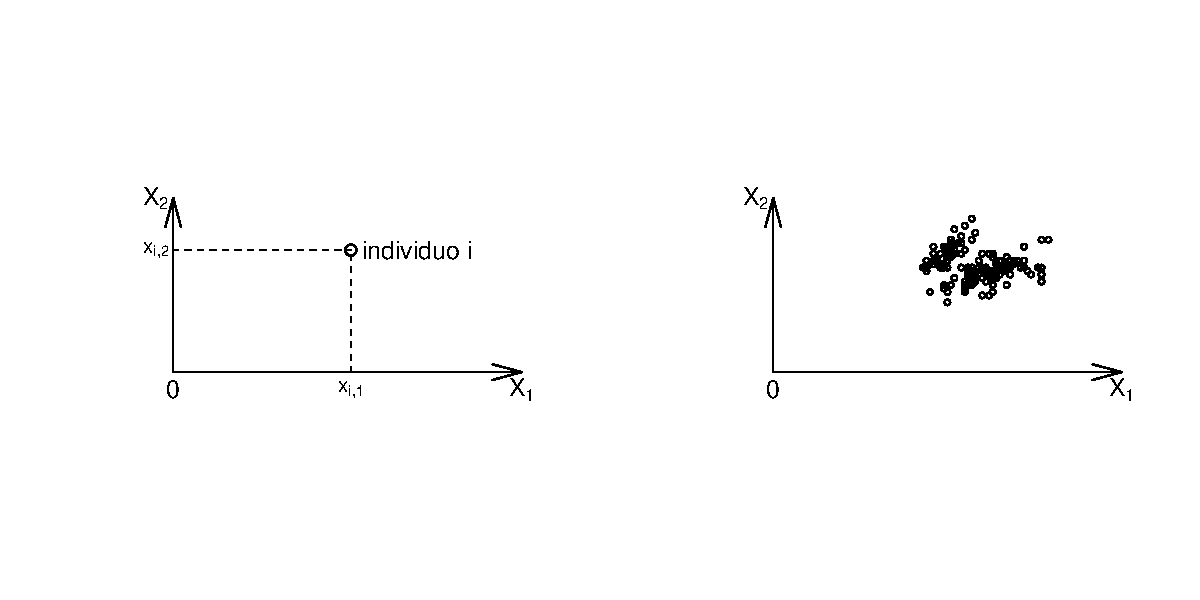
\includegraphics{dispense_pca_files/figure-latex/unnamed-chunk-1-1.pdf}

\hypertarget{trasformazione-delle-variabili-centratura-e-standardizzazione}{%
\section{Trasformazione delle variabili: centratura e standardizzazione}\label{trasformazione-delle-variabili-centratura-e-standardizzazione}}

Indichiamo con \(\bar{x_1},\dots,\bar{x_p}\) le medie delle variabili \(X_1,\dots,X_p\),
cioè le \(p\) medie delle \(p\) colonne della Tabella \ref{tab:RegrMult}, e con
\(\sigma_1^2,\dots,\sigma_p^2\) le rispettive varianze.\\
Il vettore \(\bar{x}=(\bar{x_1},\dots,\bar{x_p})\) viene chiamato \textbf{baricentro}.

\textbf{Centratura}: semplice traslazione del baricentro nell'origine
\begin{equation}
x_{ij}^{'}=x_{ij}-\bar{x_j}
\end{equation}

\begin{itemize}
\tightlist
\item
  non perdo informazione sulla distanza tra i punti (la geometria della nuvola di punti
  rimane invariata)
\item
  perdo solo informazione sul baricentro
\item
  semplifica formule e conti (da ora in poi useremo sempre dati centrati)
\end{itemize}

\textbf{Standardizzazione}: questa trasformazione porta ogni variabile ad avere varianza \(1\)
(in generale questa trasformazione viene fatta insieme alla centratura)
\begin{equation}
x_{ij}^{'}=\frac{x_{ij}-\bar{x_j}}{\sigma_j}
\end{equation}

\begin{itemize}
\tightlist
\item
  questa trasformazione rende le variabili degli scalari (numeri puri)
\item
  questa trasformazione è necessaria quando si vogliono confrontare variabili
  con differenti unità di misura (le variabili devono essere omogenee per essere confrontabili)
\item
  tutte le variabili hanno lo stesso ``peso''
\item
  cambia la distanza (la geometria) tra i punti. E' una dilatazione o contrazione.
\end{itemize}

Si veda la seguente figura per una rappresentazione grafica di dati centarti e
scalati per una matrice di dati di \(2\) variabili

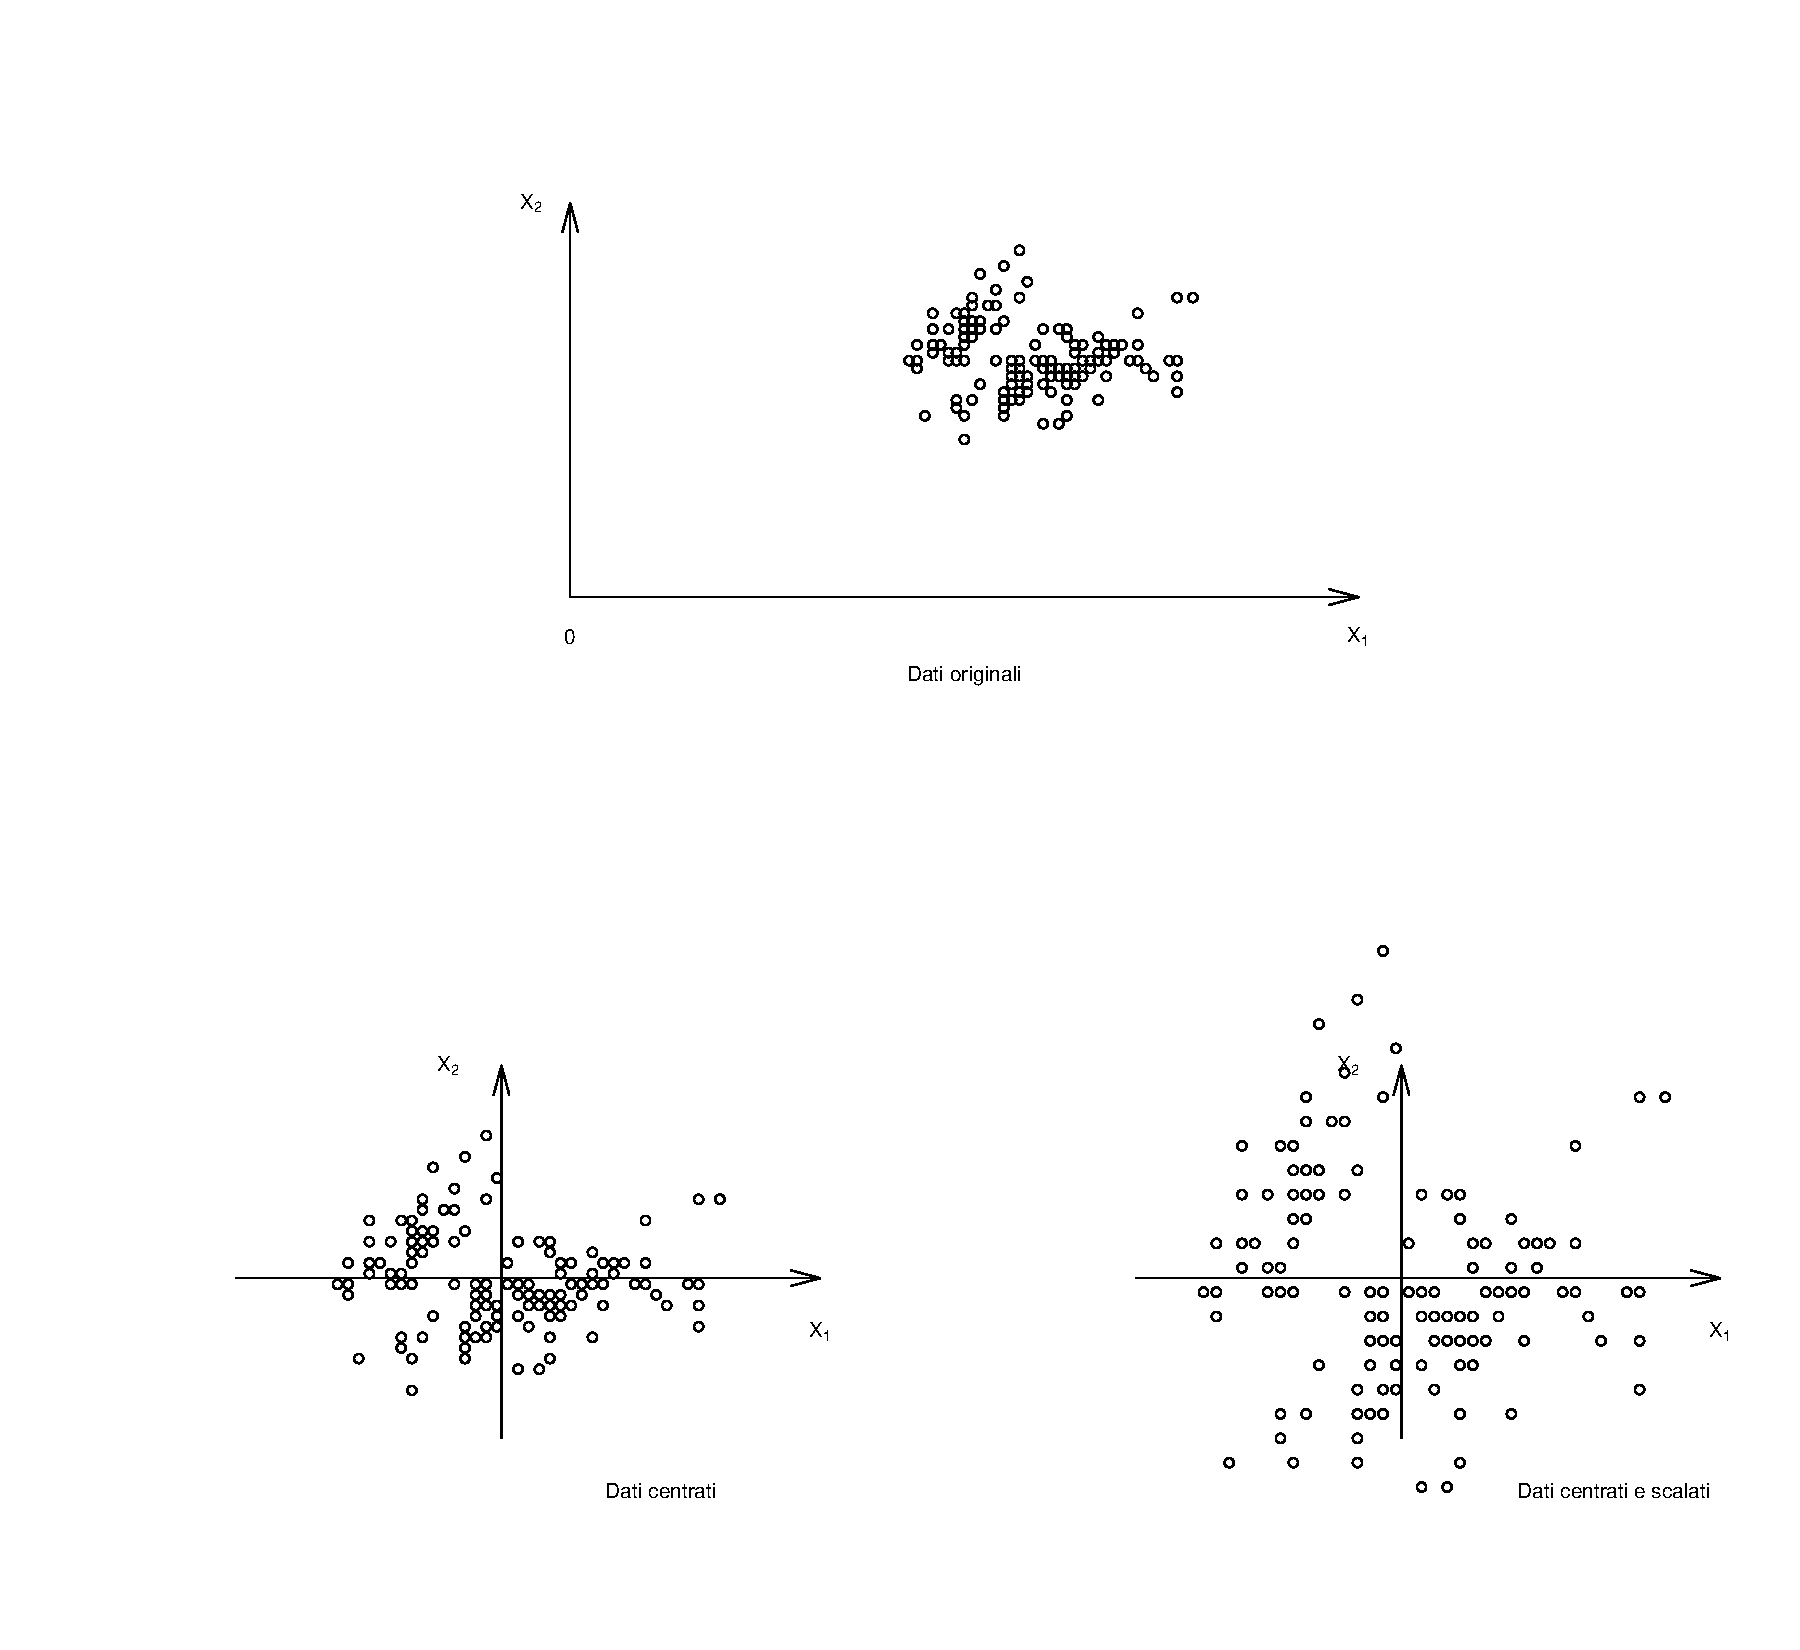
\includegraphics{dispense_pca_files/figure-latex/unnamed-chunk-2-1.pdf}

  \bibliography{book.bib}

\addcontentsline{toc}{chapter}{Bibliografia}

\end{document}
